\documentclass[tikz, border=14pt]{standalone}
\usepackage{tikz}
\usepackage{amsmath}
\usepackage{amssymb}
\usetikzlibrary{arrows.meta, positioning, fit, backgrounds, calc, decorations.pathreplacing}

%% Color palette (shared with controlled_dhgn_lstm_arch.tex)
\colorlet{Cenc}{blue!65!black}
\colorlet{Cflow}{orange!80!black}
\colorlet{Cdyn}{violet!75!black}
\colorlet{Cctrl}{red!65!black}
\colorlet{Cdec}{green!60!black}

\tikzset{
  encbox/.style={draw=Cenc, fill=Cenc!8, rounded corners=3pt, thick,
    align=center, minimum height=0.9cm, minimum width=1.4cm, font=\small},
  decbox/.style={draw=Cdec, fill=Cdec!8, rounded corners=3pt, thick,
    align=center, minimum height=0.9cm, minimum width=1.4cm, font=\small},
  flowbox/.style={draw=Cflow, fill=Cflow!10, rounded corners=3pt, thick,
    align=center, font=\small},
  latent/.style={draw=Cenc, fill=Cenc!6, circle, thick,
    inner sep=1pt, minimum size=8mm, font=\small},
  phase/.style={draw=Cdyn, fill=Cdyn!8, rounded corners=3pt, thick,
    inner sep=3pt, minimum height=8mm, font=\small},
  eqbox/.style={draw=Cdyn, fill=Cdyn!4, rounded corners=4pt, thick,
    align=center, inner sep=6pt, font=\small},
  arr/.style={-{Stealth[length=6pt, width=4.5pt]}, thick, black!70},
  flowarr/.style={{Stealth[length=6pt, width=4.5pt]}-{Stealth[length=6pt, width=4.5pt]},
    thick, Cflow},
  dim/.style={font=\scriptsize, text=black!55},
  %% Stylised Pendulum-v1 frame: cream background, rust rod, dark axle
  pics/pend/.style={code={%
    \draw[fill=brown!7!white, draw=black!50, rounded corners=1pt]
      (-0.55,-0.55) rectangle (0.55,0.55);
    \draw[line width=2.6pt, draw=red!50!brown, line cap=round] (0,0) -- (#1:0.42);
    \fill[black!75] (0,0) circle (0.05);
  }},
}

\begin{document}
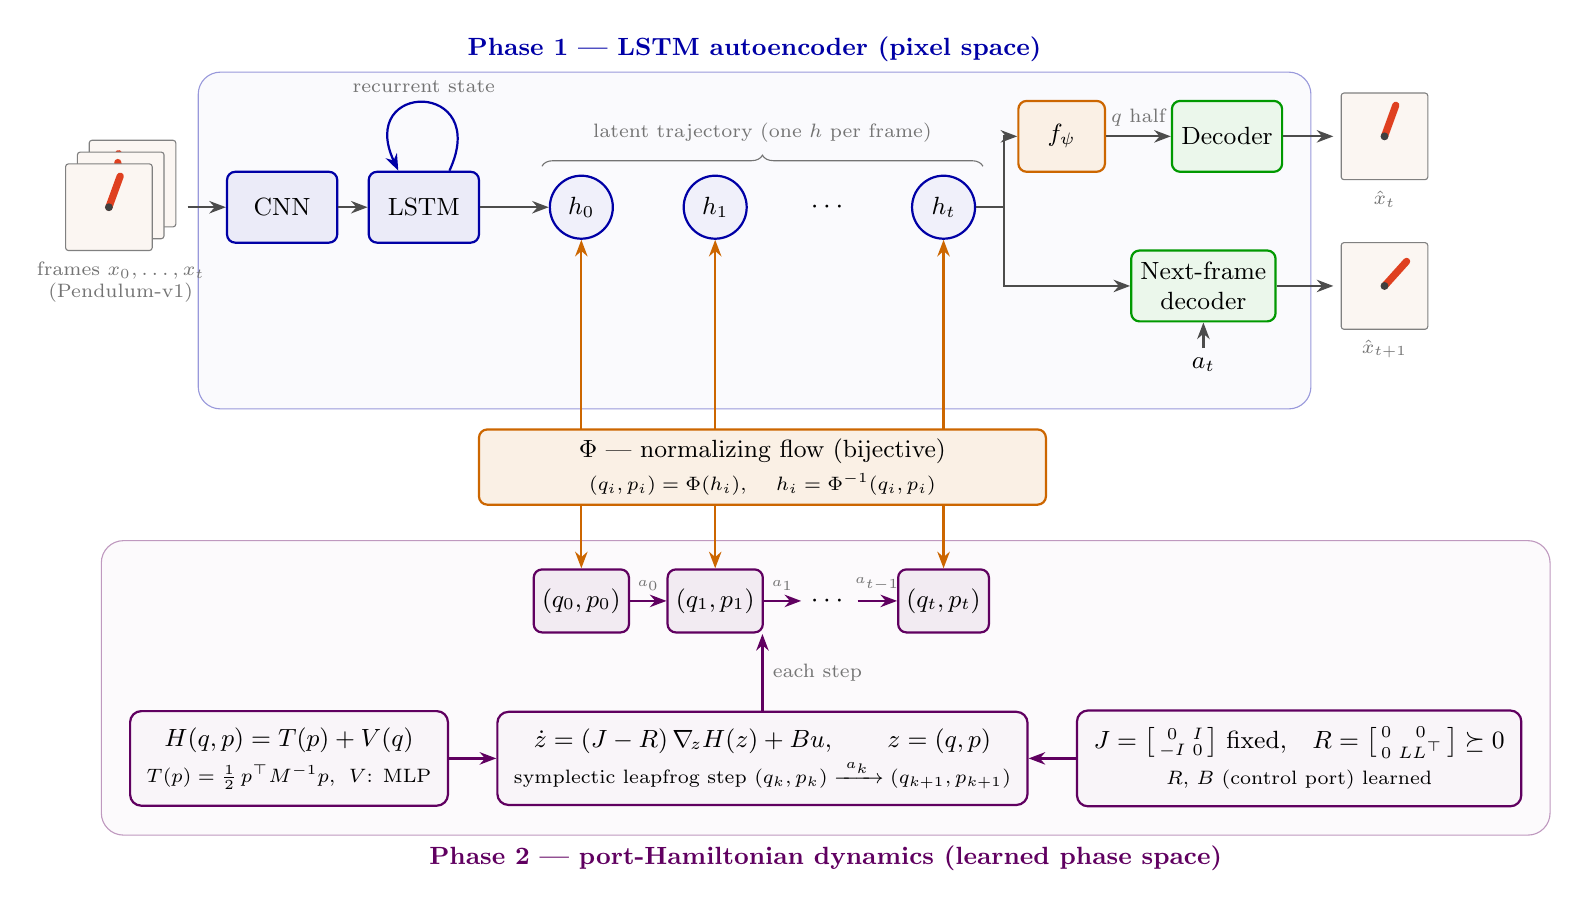
\begin{tikzpicture}

%%==========================================================================
%% TOP PATH — Phase 1 autoencoder (pixel space)
%%==========================================================================

%% Input frames (stacked to suggest the sequence)
\pic at (0.30, 0.30) {pend=115};
\pic at (0.15, 0.15) {pend=95};
\pic at (0, 0)       {pend=70};
\node[dim, align=center] at (0.15, -0.95) {frames $x_0,\dots,x_t$\\ (Pendulum-v1)};

\node[encbox] (cnn)  at (2.2, 0) {CNN};
\node[encbox] (lstm) at (4.0, 0) {LSTM};
\draw[arr, Cenc] (lstm.55) to[out=65, in=115, looseness=5]
  node[above, dim] {recurrent state} (lstm.125);

%% Latent trajectory h_0 ... h_t
\node[latent] (h0) at (6.0, 0)  {$h_0$};
\node[latent] (h1) at (7.7, 0)  {$h_1$};
\node         (hd) at (9.15, 0) {$\cdots$};
\node[latent] (ht) at (10.6, 0) {$h_t$};
\draw[decorate, decoration={brace, amplitude=4pt, raise=2pt}, black!55]
  (5.5, 0.45) -- (11.1, 0.45)
  node[midway, above=7pt, dim] {latent trajectory (one $h$ per frame)};

%% Reconstruction branch: h_t -> f_psi -> Decoder -> xhat_t
\node[flowbox, minimum height=0.9cm, minimum width=1.1cm] (fpsi) at (12.1, 0.9) {$f_\psi$};
\node[decbox]  (dec)  at (14.2, 0.9) {Decoder};
\pic at (16.2, 0.9) {pend=70};
\node[dim] at (16.2, 0.1) {$\hat{x}_t$};

%% Next-frame branch: (h_t, a_t) -> next-frame decoder -> xhat_{t+1}
\node[decbox] (nfd) at (13.9, -1.0) {Next-frame\\decoder};
\node[font=\small] (act) at (13.9, -2.0) {$a_t$};
\pic at (16.2, -1.0) {pend=48};
\node[dim] at (16.2, -1.8) {$\hat{x}_{t+1}$};

%% Top-path arrows
\draw[arr] (1.0, 0) -- (cnn);
\draw[arr] (cnn) -- (lstm);
\draw[arr] (lstm) -- (h0);
\draw[arr] (ht.east) -- ++(0.35, 0) |- (fpsi.west);
\draw[arr] (fpsi) -- node[above, dim] {$q$ half} (dec);
\draw[arr] (dec) -- (15.55, 0.9);
\draw[arr] (ht.east) -- ++(0.35, 0) |- (nfd.west);
\draw[arr] (act) -- (nfd.south);
\draw[arr] (nfd) -- (15.55, -1.0);

%%==========================================================================
%% MIDDLE — normalizing flow Phi between latent and phase space
%%==========================================================================

%% (the Phi band itself is drawn after the crossing arrows, so it sits on top)

%%==========================================================================
%% BOTTOM PATH — Phase 2 port-Hamiltonian dynamics (learned phase space)
%%==========================================================================

\node[phase] (qp0) at (6.0, -5.0)  {$(q_0, p_0)$};
\node[phase] (qp1) at (7.7, -5.0)  {$(q_1, p_1)$};
\node        (qpd) at (9.15, -5.0) {$\cdots$};
\node[phase] (qpt) at (10.6, -5.0) {$(q_t, p_t)$};

\draw[arr, Cdyn] (qp0) -- node[above, dim, font=\tiny] {$a_0$} (qp1);
\draw[arr, Cdyn] (qp1) -- node[above, dim, font=\tiny] {$a_1$} (qpd);
\draw[arr, Cdyn] (qpd) -- node[above, dim, font=\tiny] {$a_{t-1}$} (qpt);

%% Flow crossings h_i <-> (q_i, p_i), passing through the Phi band
\draw[flowarr] (h0) -- (qp0);
\draw[flowarr] (h1) -- (qp1);
\draw[flowarr] (ht) -- (qpt);

%% Normalizing flow band (drawn after the arrows so it covers their midsections)
\node[flowbox, minimum width=7.2cm, inner xsep=12pt] (phi) at (8.3, -3.3)
  {$\Phi$ --- normalizing flow (bijective)\\[1pt]
   {\scriptsize $(q_i, p_i) = \Phi(h_i)$, \quad $h_i = \Phi^{-1}(q_i, p_i)$}};

%% Port-Hamiltonian machinery
\node[eqbox] (ode) at (8.3, -7.0)
  {$\dot{z} = (J - R)\,\nabla_{\!z} H(z) + B u, \qquad z = (q, p)$\\[2pt]
   {\scriptsize symplectic leapfrog step $(q_k, p_k) \xrightarrow{\;a_k\;} (q_{k+1}, p_{k+1})$}};

\node[eqbox, anchor=east] (ham) at ([xshift=-6mm]ode.west |- ode)
  {$H(q,p) = T(p) + V(q)$\\[2pt]
   {\scriptsize $T(p) = \tfrac{1}{2}\, p^{\top} M^{-1} p$,\; $V$: MLP}};

\node[eqbox, anchor=west] (struct) at ([xshift=6mm]ode.east |- ode)
  {$J = \left[\begin{smallmatrix} 0 & I \\ -I & 0 \end{smallmatrix}\right]$ fixed,\quad
   $R = \left[\begin{smallmatrix} 0 & 0 \\ 0 & LL^{\top} \end{smallmatrix}\right] \succeq 0$\\[2pt]
   {\scriptsize $R$, $B$ (control port) learned}};

\draw[arr, Cdyn] (ham) -- (ode);
\draw[arr, Cdyn] (struct) -- (ode);
\draw[arr, Cdyn] (ode.north) -- node[right, dim] {each step} (8.3, -5.42);

%%==========================================================================
%% BACKGROUND GROUPING
%%==========================================================================
\begin{scope}[on background layer]
  \node[draw=Cenc!40, fill=Cenc!2, rounded corners=8pt, inner sep=10pt,
    fit=(cnn)(lstm)(h0)(ht)(fpsi)(dec)(nfd)(act),
    label={[Cenc, font=\small\bfseries]above:%
      Phase 1 --- LSTM autoencoder (pixel space)}] {};
  \node[draw=Cdyn!40, fill=Cdyn!2, rounded corners=8pt, inner sep=10pt,
    fit=(qp0)(qpt)(ham)(ode)(struct),
    label={[Cdyn, font=\small\bfseries]below:%
      Phase 2 --- port-Hamiltonian dynamics (learned phase space)}] {};
\end{scope}

\end{tikzpicture}
\end{document}
